\chapter{Metodología}
\label{ch:metodologia}

\section{Definición de la metodología}

El desarrollo de este proyecto combina dos metodologías: Ulrich y Eppinger (UE), para la 
fase de definición del sistema, y el Modelo en V, para su construcción y verificación. Esta 
sección presenta cada metodología por separado, la cual explica qué es cada una, por qué se 
utiliza y en qué consisten sus etapas y cierra con la justificación de por qué se combinan en lugar 
de aplicar una sola de forma exclusiva.

\subsection{Metodología de Ulrich y Eppinger}

UE es un marco ampliamente utilizado en ingeniería de diseño que estructura el desarrollo de un 
producto o sistema desde una perspectiva centrada en las necesidades reales de sus usuarios \cite{Cite11}. 
Su aporte principal es ordenar el proceso de toma de decisiones, la cual parte de información 
cualitativa del problema, la convierte en especificaciones y de ahí deriva conceptos de solución 
comparables entre sí. Esto permite mantener trazabilidad desde el inicio, ya que cada decisión 
técnica puede justificarse mediante la necesidad y la métrica que la originaron \cite{Cite11}.

Se utiliza UE en este proyecto porque su fortaleza es precisamente la que exige la etapa inicial 
del desarrollo, en convertir los deseos expresados por el equipo en una lista de necesidades 
priorizada, esas necesidades en métricas medibles con valores objetivo y marginales, y estas
en conceptos de solución comparables para cada uno de los cinco módulos funcionales del sistema. 


\newpage

El proceso de esta metodología consta de las siguientes etapas \cite{Cite11}:

\begin{enumerate}
  \item Identificación de las necesidades del cliente: recolectar información cruda de los 
  usuarios, interpretarla como necesidades, organizarla jerárquicamente y ponderar su importancia 
  relativa.
  \item Establecimiento de especificaciones objetivo: elaborar la lista de métricas ligadas a 
  cada necesidad, recabar información de contexto, y fijar valores marginales y objetivos para cada 
  métrica.
  \item Generación de conceptos: búsqueda externa de soluciones existentes y búsqueda interna 
  de alternativas técnicas para cada subsistema.
  \item Selección del concepto: comparación estructurada de las alternativas generadas mediante 
  matrices de filtrado y evaluación, hasta escoger un concepto por subsistema.
\end{enumerate}

Este proyecto aplica formalmente solo para estas etapas de la metodología de Ulrich y Eppinger, ya 
que estas son las que corresponden a un sistema de ingeniería que aún no ha sido construido y para 
el cual se debe decidir, qué solución implementar por módulo. 

\subsection{Metodología Modelo en V}

El Modelo en V (V-Model) es una metodología de diseño en ingeniería que vincula de forma explícita 
cada etapa de definición y diseño de un sistema con una etapa de verificación equivalente. Fue 
presentado originalmente por Forsberg y Mooz \cite{Cite7} como una representación del ciclo de vida de un 
proyecto, y formalizado posteriormente para sistemas mecatrónicos en la norma alemana VDI 2206, ampliada 
por Gausemeier y Moehringer \cite{Cite8}. 

Se utiliza el Modelo en V en este proyecto porque el sistema desarrollado es, por naturaleza, 
mecatrónico que es precisamente el escenario para el que la norma VDI 2206 fue concebida \cite{Cite8}. 
Además, los objetivos específicos del proyecto están definidos mediante indicadores 
cuantitativos de desempeño, es decir, criterios que solo pueden confirmarse mediante un proceso de 
prueba explícito y trazable hasta el requisito que los originó. El Modelo en V provee esa 
trazabilidad de forma nativa.

El modelo se organiza en dos ramas \cite{Cite7} \cite{Cite8}\\:

Rama izquierda (especificación y diseño), de forma descendente:

\begin{enumerate}
    \item Requisitos del sistema, los cuales se toman de lo elaborado en la metodología UE.
    \item Arquitectura del sistema, que corresponde a la integración de los módulos funcionales.
    \item Diseño detallado por subsistema.
    \item Implementación y prototipado.
\end{enumerate}

Rama derecha (verificación), ascendente: 

\begin{enumerate}
    \item Pruebas unitarias por subsistema, para verificar la implementación y prototipado. 
    \item Pruebas de integración entre módulos, para verificar el diseño por subsistema. 
    \item Validación del sistema completo contra los requisitos originales.
\end{enumerate}

La correspondencia horizontal entre cada nivel de la rama izquierda y su contraparte en la rama 
derecha constituye la trazabilidad del modelo, y es su característica distintiva frente a otras 
metodologías de diseño: cada decisión de diseño tiene, desde su origen, una prueba definida que 
confirmará si fue correcta. 

Se presenta en la Figura \ref{fig:metodologia} un diagrama de flujo que explica la metodología en 
V para una mejor referencia \cite{Cite8}.

\begin{figure}[H]
    \centering
    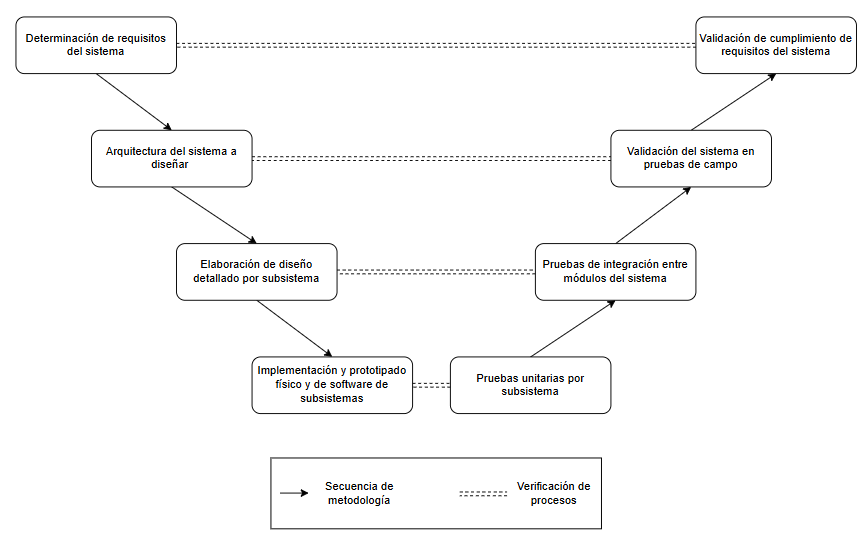
\includegraphics[width=1.0\textwidth]{fig/modelo_v.png}
    \caption{Diagrama de flujo de la metodología en V}
    \label{fig:metodologia}

\end{figure}

\newpage

\subsection{Justificación de uso mixto de metodologías}

UE y el Modelo en V no son metodologías competidoras sino complementarias, y por eso se combinan 
en lugar de aplicar una sola de forma exclusiva. UE no incluye, en sus etapas 1 a 4, una estructura 
de verificación en profundidad, mientras que Modelo en V, por su parte, no incluye 
herramientas propias de generación y selección de conceptos, ya que este asume que el conjunto de 
requisitos con el que arranca la rama izquierda ya existe. Ninguna de las dos, por separado, 
cubre el proceso completo que este proyecto necesita, pero en conjunto sí lo hacen. 

En este proyecto, la división del trabajo queda en que la metodología UE determina qué construir, en este caso 
necesidades, métricas, especificaciones y la selección del concepto a implementar por cada uno 
de los módulos funcionales del sistema. El  Modelo en V determina cómo se construye y cómo se 
verifica lo seleccionado. El punto de entrega entre ambas metodologías es exactamente el concepto 
seleccionado al final de la etapa 4 de UE, que se convierte en el "Requisitos del sistema" con el 
que arranca la rama izquierda del Modelo en V.

\newpage

\section{Procedimiento para obtener necesidades, métricas y especificaciones}

\subsection{Necesidades del cliente}

La lista de necesidades se construyó a partir de una entrevista formal realizada al equipo
del grupo MACS responsable del proyecto, en lugar de partir de una descripción del problema
previamente redactada por los profesores, con el fin de evitar el sesgo del problema percibido.
La guía de entrevista y las respuestas obtenidas se incluyen en el Apéndice [A]. Siguiendo el
procedimiento de UE, las afirmaciones de la entrevista se interpretaron primero como una
lista inicial de necesidades individuales. Esta lista se organizó después en una jerarquía
de necesidades primarias y secundarias, donde cada necesidad primaria generaliza un grupo de
necesidades secundarias afines, agrupadas por similitud temática. Durante esta organización
se consolidaron además dos parejas de necesidades secundarias que expresaban, en esencia,
el mismo requisito, resultando en una lista final de necesidades. 

Seguidamente, a cada necesidad secundaria se le asignó un nivel de importancia del 1 al 5, siguiendo la
escala: 1, no se realiza en esta versión del sistema; 2, funcional pero de última prioridad;
3, necesario a menor escala (deseable); 4, importante aunque no obligatorio de forma explícita;
y 5, imprescindible (obligatorio para el proyecto). La importancia se asignó según cómo los 
propios entrevistados calificaron cada necesidad, sin introducir criterio adicional del equipo de 
diseño.

Esta jerarquía de necesidades primarias y secundarias se resume en la Tabla \ref{tab:necesidades}.

\newpage

\begin{longtable}{|c|p{12cm}|c|}
\caption{Lista jerárquica de necesidades primarias y secundarias del sistema} \label{tab:necesidades} \\
\hline
\textbf{N.\textordmasculine{}} & \textbf{Necesidad} & \textbf{Importancia} \\
\hline
\endfirsthead

\multicolumn{3}{c}{\tablename\ \thetable\ -- continuación} \\
\hline
\textbf{N.\textordmasculine{}} & \textbf{Necesidad} & \textbf{Importancia} \\
\hline
\endhead

\hline
\multicolumn{3}{r}{continúa en la siguiente página} \\
\endfoot

\hline
\endlastfoot

\textbf{1} & \textbf{El sistema debe operar y coordinar la flota de USV de forma autónoma, con la precisión de navegación necesaria para el cumplimiento confiable de la misión.} & \\ \hline
 & El sistema debe ejecutar misiones de forma autónoma, con conciencia del entorno operativo durante la navegación. & 5 \\ \hline
 & El operador debe poder transferir el control de la embarcación al sistema embarcado durante la misión. & 5 \\ \hline
 & El sistema debe coordinar dos USV mediante navegación por waypoints, como primera demostración de operación multivehículo. & 5 \\ \hline
 & La arquitectura debe permitir, a futuro, extender la coordinación a misiones múltiples y simultáneas. & 1 \\ \hline

\textbf{2} & \textbf{El sistema debe registrar y transmitir de forma continua y completa los datos de la misión.} & \\ \hline
 & El sistema registra la trayectoria, las señales de control y el consumo energético de cada USV durante la misión. & 5 \\ \hline
 & El sistema transmite en tiempo real telemetría de posición, orientación, velocidad y RPM. & 5 \\ \hline
 & El sistema transmite las imágenes capturadas como parte de los datos de la misión. & 3 \\ \hline

\textbf{3} & \textbf{El sistema permite definir y ajustar los criterios de éxito según los objetivos de cada misión.} & 5\\ \hline

\textbf{4} & \textbf{La integración del hardware nuevo no debe comprometer la integridad física ni la estabilidad de la embarcación existente.} & \\ \hline
 & La integración no debe modificar estructura, flotabilidad ni propulsores existentes. & 5 \\ \hline
 & La ubicación de los componentes no debe comprometer el centro de gravedad. & 5 \\ \hline
 & Los conectores de los nuevos componentes deben ser físicamente accesibles. & 4 \\ \hline

\textbf{5} & \textbf{El sistema debe mantener una comunicación confiable y de suficiente alcance entre los USV y la estación base.} & \\ \hline
 & La comunicación USV--estación base debe ser tipo pseudo-WIFI. & 5 \\ \hline
 & El sistema debe mantener disponible el enlace de radio como canal redundante. & 5 \\ \hline

\textbf{6} & \textbf{El sistema debe contar con mecanismos redundantes para la recuperación de la embarcación ante fallos.} & 5\\ \hline

\textbf{7} & \textbf{El sistema debe incorporar sensores de percepción para la captura de información ambiental durante la misión.} & \\ \hline
 & El sistema permite la incorporación de un sensor LIDAR o una cámara. & 4 \\ \hline
 & El sistema permite la captura de imágenes durante la navegación. & 3 \\ \hline
 & La medición de calidad del agua es una necesidad a futuro, fuera del alcance actual. & 1 \\ \hline

\end{longtable}

La priorización muestra que las necesidades secundarias más críticas corresponden al registro obligatorio de datos de misión y la definición del criterio de
éxito de la misión, las restricciones físicas de integración en el casco, y la comunicación
primaria y redundante entre los USV y la estación base. Esto confirma que el proyecto está
orientado a la verificación medible del desempeño, reforzando la pertinencia del Modelo en V
para la fase de construcción.

Dentro de la escala de importancia, el valor 1 identifica necesidades secundarias que el
equipo de MACS mencionó como relevantes para el sistema, pero que, por definición de la
escala, no se implementan en esta versión del proyecto. Estas son necesidades reales,
expresadas por el cliente durante la entrevista, cuya ejecución se proyecta a futuro. En este
proyecto corresponden a la extensión de la coordinación a misiones múltiples y simultáneas
(primaria de operación autónoma) y a la medición de calidad del agua (primaria de sensores
de percepción). Ambas quedan, en consecuencia, excluidas del proceso de generación de
métricas, ya que no forman parte del alcance que este proyecto debe validar; se conservan en
la lista completa para preservar la trazabilidad del levantamiento con el cliente y dejar
constancia de ellas como trabajo futuro.


\newpage

\subsection{Lista de especificaciones del sistema}

Seguidamente, se procede a delimitar las métricas según las necesidades del cliente identificadas.
Antes de fijar valores objetivo, se investigaron los conceptos técnicos que determinan qué valores 
son razonables para las métricas más críticas. 

Antes de fijar valores objetivo, se investigaron los conceptos técnicos que determinan qué valores
son razonables para las métricas más críticas, ya sea para fijar un valor objetivo cuando la
necesidad no lo especificaba, o para confirmar que el valor ya declarado por el cliente es
técnicamente alcanzable con la tecnología disponible.

\begin{itemize}
    \item Posicionamiento(M4). GNSS estándar sin corrección da 3–5 m \cite{Cite13}, 
    insuficiente para el marginal de $\leq$2 m. RTK da 1–2 cm \cite{Cite13}, y un sistema comparable con 
    RTK y percepción LIDAR logró en campo 0.046 m de error promedio y 0.12 m máximo \cite{Cite9}, el cual 
    respalda 0.5 m como ideal de M4.
    \item Comunicación (M5, M8). Los radios RFD900x ya presentes en la plataforma alcanzan $\geq$40 km 
    en línea de vista y hasta 500 kbps, por lo que el ideal de M8 (1–2 km) es alcanzable con 
    holgura. La latencia de M5 no está publicada en su hoja de datos, por lo que se medirá de forma
    empírica \cite{Cite10}.
    \item Latencia de software (M3, M5). Un estudio que compara MAVROS–MAVLink frente a DDS 
    nativo en vehículos autónomos reporta diferencias de latencia del orden de cientos de microsegundos, 
    muy por debajo de los marginales de 500 ms y de 1 s, confirmando que ambos son 
    alcanzables con el stack ROS2 ya definido \cite{Cite12}.
\end{itemize}

Siguiendo el procedimiento oficial de UE \cite{Cite11} cada necesidad se 
tradujo en una o más métricas verificables, ligadas explícitamente a su necesidad de origen y a 
la importancia heredada de esta en la Tabla \ref{tab:necesidades}. Los valores objetivo se expresan, donde la información 
lo permite, como valor marginal y valor ideal, siguiendo la 
directriz de que un valor único y exacto solo se usa cuando es obligatorio o no puede establecerse 
de otra forma. Estas métricas y valores objetivo se resumen en la Tabla \ref{tab:metricas}, que 
constituye la lista de especificaciones del sistema.

\newpage

% ------------------------------------------------------------
% TABLA 3.2 -- Métricas y valores objetivo (retrato, longtable)
% ------------------------------------------------------------
\footnotesize
\setlength{\tabcolsep}{5pt}
\begin{longtable}{|c|p{1.3cm}|p{3.1cm}|c|p{1cm}|p{1.6cm}|p{1.7cm}|p{3.6cm}|}
\caption{Métricas y valores marginales e ideales del sistema} \label{tab:metricas} \\
\hline
\textbf{M.\textordmasculine{}} & \textbf{N.\textordmasculine{}} & \textbf{Métrica} & \textbf{Imp.} & \textbf{Unid.} & \textbf{Val. marginal} & \textbf{Val. ideal} & \textbf{Verificación} \\
\hline
\endfirsthead
 
\multicolumn{8}{c}{\tablename\ \thetable\ -- continuación} \\
\hline
\textbf{M.\textordmasculine{}} & \textbf{N.\textordmasculine{}} & \textbf{Métrica} & \textbf{Imp.} & \textbf{Unid.} & \textbf{Val. marginal} & \textbf{Val. ideal} & \textbf{Verificación} \\
\hline
\endhead
 
\hline
\multicolumn{8}{r}{continúa en la siguiente página} \\
\endfoot
 
\hline
\endlastfoot
 
M1 & 1,3 & Tasa de pruebas funcionales superadas & 5 & \% & $\geq$90 & $\geq$95 & Mínimo 10 ciclos por vehículo (arranque, comunicación autopiloto--ordenador a bordo, respuesta a comandos), documentado en el reporte técnico de integración. \\ \hline
M2 & 2,7 & Porcentaje de disponibilidad de sensores & 5 & \% & $\geq$90 & $\geq$95 & Medida durante misiones continuas de al menos 30 min en laboratorio; documentada en el set de datos de prueba. \\ \hline
M3 & 2,7 & Latencia de adquisición & 5 & ms & $\leq$500 & $\leq$500 & Medida por muestra durante las mismas misiones de 30 min; documentada en el set de datos de prueba. \\ \hline
M4 & 1 & Error de trayectoria & 5 & m & $\leq$2 & $<$0.5 & Medido en misiones de al menos 20 min con dos USV ejecutando waypoints (simulación y prueba de concepto); registrado en logs de misión y trayectorias. \\ \hline
M5 & 5 & Latencia de comunicación & 5 & s & $\leq$1 & $\leq$0.8 & Medida durante las mismas misiones de 20 min de coordinación por waypoints; documentada en el reporte técnico de comunicaciones y navegación. \\ \hline
M6 & 1,3 & Tasa de éxito de misión & 5 & \% & $\geq$85 & $\geq$100 & Evaluada en al menos 3 pruebas de integración independientes, con al menos 2 puntos de muestreo por USV por misión; documentada en el reporte de análisis de resultados. \\ \hline
M7 & 4 & Peso de componentes añadidos & 5 & kg & $\leq$5 & $\leq$4 & Pesaje físico de todos los componentes antes de integración. \\ \hline
M8 & 5 & Alcance de comunicación & 5 & m & $\geq$100 & $\geq$1000 & Pruebas de campo a distancia creciente hasta pérdida de enlace. \\ \hline
M9 & 2,7 & Frecuencia de imágenes & 2 & Hz & $\approx$1 & $\approx$2 & Marca de tiempo de los cuadros capturados. \\ \hline
M10 & 6 & Número de mecanismos de recuperación & 5 & \# & $\geq$3 & $\geq$4 & Desconexión intencional de cada canal, confirmando la conmutación (\textit{failover}). \\ \hline
M11 & 4 & Modificación del casco y Estabilidad (GM) & 5 & Bin. & Sí & No & Inspección del casco tras la integración y cálculo de altura metacéntrica (GM) del casco cargado vs.\ vacío.\\ \hline
M12 & 4 & Accesibilidad de conectores & 4 & Bin. & Sí & Sí & Verificación de acceso físico sin desmontaje mayor. \\ \hline

\end{longtable}
\setlength{\tabcolsep}{6pt}
\normalsize

De las métricas investigadas en esta etapa, la investigación cumplió dos propósitos distintos.
Para M4 y M8, el valor objetivo ya había sido establecido directamente por el cliente durante
la entrevista (Apéndice [A]). La investigación, en ambos casos, solo
confirmó que la tecnología seleccionada puede alcanzarlo con holgura. Para M3 y M5, en
cambio, ni la entrevista ni la necesidad de origen incluían un valor numérico, por lo que la
investigación buscó establecerlo, y en ambos casos se confirmó la viabilidad del umbral definido
por el equipo mediante literatura sobre latencia en ROS2.

Las métricas M7, M9, M10, M11 y M12
tampoco requirieron ningún tipo de investigación adicional, ya que el peso máximo de componentes,
la frecuencia de imágenes, el número de mecanismos de recuperación y las dos condiciones
binarias fueron indicados directamente por el equipo de MACS durante la entrevista (Apéndice
[A]), aunque esos valores se registran únicamente en la Tabla 3.2 y
no como necesidades independientes en la Tabla 3.1. Las métricas M1, M2 y M6, por su parte,
no cuentan con un valor equivalente ni en la entrevista ni en la literatura consultada, ya que
se establecieron como criterio de aceptación definido por el propio equipo de desarrollo del
proyecto, ante la ausencia de un estándar externo aplicable a un sistema de este alcance.

\newpage

Para verificar la trazabilidad completa entre las necesidades del cliente y las métricas
definidas, se construyó una matriz de correspondencia entre las siete necesidades primarias
de la Tabla \ref{tab:necesidades} y las doce métricas de la Tabla \ref{tab:metricas}, tomando como base la columna de
primarias ya asignada a cada métrica en dicha tabla. Esta correspondencia se
resume en la Figura \ref{fig:matriz}.

\begin{figure}[H]
    \centering
    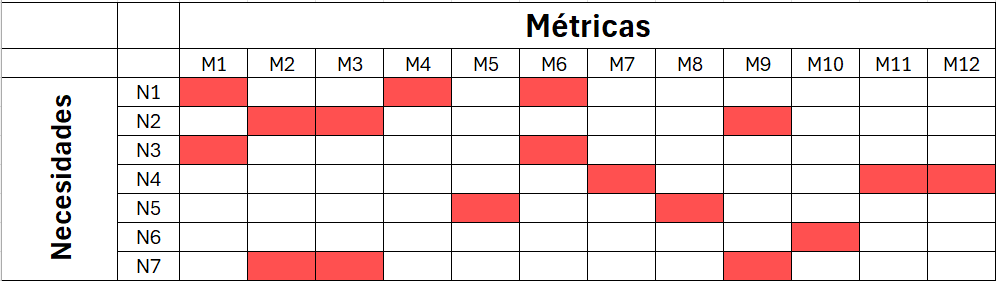
\includegraphics[width=1.0\textwidth]{fig/matriz.png}
    \caption{Matriz de necesidades y métricas del sistema}
    \label{fig:matriz}

\end{figure}

\subsection{Selección del concepto ganador}

Siguiendo la metodología de conceptualización presentada en el curso, basada en el proceso
de generación de conceptos de Ulrich y Eppinger, la primera etapa consiste en dividir el
problema de diseño en subproblemas más manejables mediante una descomposición funcional.
Este proceso parte de una caja negra que define, de forma tentativa, las entradas y salidas de
energía, material e información del sistema, y continúa de manera iterativa y piramidal hasta
obtener subfunciones que puedan abordarse de manera independiente.

En este proyecto, se tiene la Figura \ref{fig:caja-negra}, que a partir de ella se obtuvo la 
descomposición funcional de primer nivel en la Figura \ref{fig:descomposicion-funcional}, que organiza las subfunciones del
sistema en dos flujos: uno de energía y estructura, y otro de información y control. De las
once subfunciones identificadas, tres corresponden a elementos ya resueltos por la plataforma
existente y no requieren un proceso de búsqueda de conceptos. Las ocho restantes sí
lo requieren, y son el punto de partida de la búsqueda de conceptos, externa e interna, que se
desarrolla en la siguiente sección.

\begin{figure}[htbp]
    \centering
    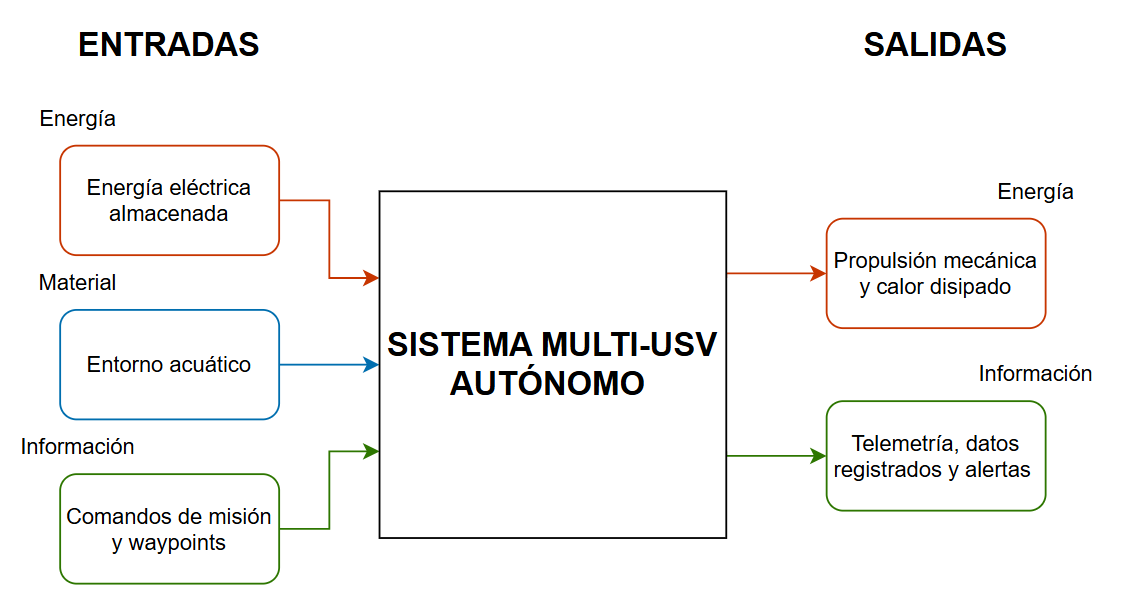
\includegraphics[width=\textwidth]{fig/caja_negra.png}
    \caption{Caja negra del sistema a diseñar}
    \label{fig:caja-negra}
\end{figure}

\begin{figure}[htbp]
    \centering
    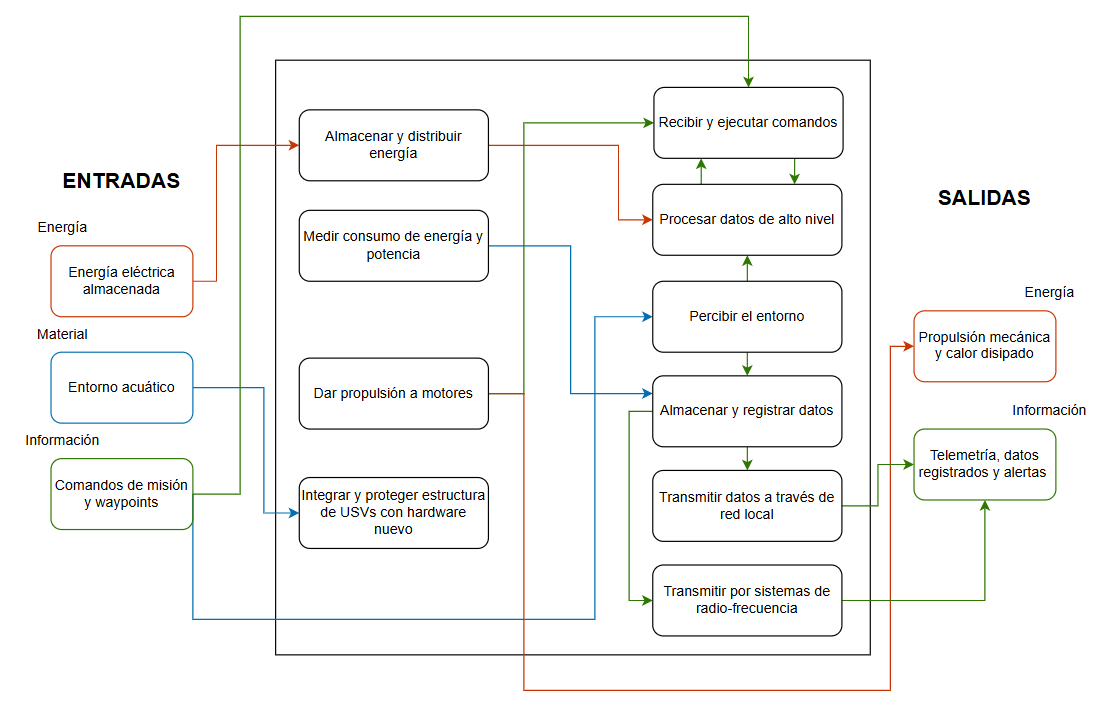
\includegraphics[width=\textwidth]{fig/descomposicion.png}
    \caption{Descomposición funcional de primer nivel del sistema a diseñar}
    \label{fig:descomposicion-funcional}
\end{figure}

\newpage

Para cada subfunción que lo requiere, se realiza una búsqueda de conceptos por dos vías, la
interna, que es a partir del conocimiento y la experiencia del equipo con la plataforma existente, y
la externa, mediante literatura técnica y análisis comparativo de productos disponibles. En esta
etapa no se aplica ningún filtro ni selección, ya que solo se busca generar el listado más exhaustivo
posible de alternativas, que se evaluarán formalmente en la etapa de selección de conceptos.

\subsubsection*{Recibir y ejecutar comandos}

\begin{itemize}
    \item \textbf{Pixhawk 6X} \\
    \textit{Justificación:} Es el controlador de vuelo ya integrado y en uso en la plataforma USV
    del grupo MACS, corriendo ArduPilot (ArduRover) sobre el stack ROS2/MAVROS ya definido.
    Ofrece redundancia triple de IMU con dominios de sensores completamente aislados (buses y
    alimentación separados) y soporte Ethernet nativo. Representa
    además la opción de menor riesgo de integración, al no requerir cambios de firmware,
    drivers ni configuración existente \cite{Cite14}. \\

    \item \textbf{Pixhawk 6C} \\
    \textit{Justificación:} Alternativa dentro de la misma familia y estándar Pixhawk, compatible
    con ArduPilot 4.3+ y con el stack ya definido. Procesador STM32H743 a 480 MHz, redundancia
    doble de IMU (ICM-42688-P + BMI088) con 34.6 g en carcasa plástica \cite{Cite14}. \\

    \item \textbf{Pix32 v6} \\
    \textit{Justificación:} Variante modular de la familia Pixhawk 6C, con controlador y placa
    base separados y conectados por un conector de 100 pines. Mismo procesador STM32H743
    a 480 MHz, redundancia doble de IMU, 36 g de peso (solo módulo
    FC). Es la opción más económica y compacta de la familia Pixhawk-estándar
    si se prioriza costo sobre redundancia \cite{Cite14} \cite{Cite15}. \\
\end{itemize}

\subsubsection*{Procesar datos de alto nivel (ordenador a bordo)}

\begin{itemize}
    \item \textbf{Raspberry Pi 4 (8 GB)} \\
    \textit{Justificación:} SBC de bajo costo y bajo consumo (3--8 W), con
    soporte nativo de ROS 2 en ARM64. Adecuado para bridging de sensores,
    teleoperación y pipelines de percepción ligeros. No cuenta con acelerador de IA dedicado,
    lo que limita el procesamiento denso de datos LIDAR/cámara en tiempo real y podría
    comprometer el cumplimiento de M2 y M3 si el
    pipeline de percepción resulta exigente \cite{Cite16}. \\

    \item \textbf{Raspberry Pi 5 (8 GB)} \\
    \textit{Justificación:} Mejora de CPU respecto al Pi 4 (Cortex-A76 a 2.4 GHz), mismo
    ecosistema ARM64/ROS 2, con la opción de un Hailo-8L (AI Kit, 13 TOPS) para inferencia
    ligera con consumo de 5--15 W. Sigue siendo limitado frente a
    modelos de percepción pesados sin el kit adicional de IA \cite{Cite16}. \\

    \item \textbf{Jetson Orin Nano 8 GB} \\
    \textit{Justificación:} GPU Ampere de 1024 núcleos con 32 Tensor cores, hasta 67 TOPS
    (INT8 disperso), con soporte nativo de Isaac ROS (cuVSLAM, Nvblox), con un consumo de 7--25 W. Es la opción
    recomendada en la literatura consultada para cargas de percepción exigentes en robots
    móviles \cite{Cite16}. \\

    \item \textbf{Intel NUC 13 Pro} \\
    \textit{Justificación:} Arquitectura x86 nativa, con mejor soporte de SDKs propietarios de
    sensores (Ouster, Velodyne, ZED) y mayor rendimiento de un solo hilo para tareas de
    planificación CPU-intensivas. Consumo considerablemente mayor (15--45 W) y requiere
    alimentación de 19--20 V con conversor DC-DC adicional, lo que complica su integración en
    el presupuesto energético del USV \cite{Cite16}. \\
\end{itemize}

\subsubsection*{Percibir el entorno}
\begin{itemize}
  \item \textbf{LIDAR SLAMTEC RPLIDAR A3} \\
  \textit{Justificación:} LIDAR 2D de barrido 360°, alcance $\approx$25\,m, $\approx$170\,g y 
  $\approx$\$300, con drivers ROS2 nativos y amplio uso en prototipado académico. Es la opción 
  más económica y ligera, aunque su clasificación IP20 implica que carece de protección contra 
  agua y polvo, por lo que en un USV requeriría una carcasa adicional \cite{Cite17}. \\

  \item \textbf{LIDAR Livox Mid-360} \\
  \textit{Justificación:} LIDAR 3D de campo de visión 360°$\times$59°, $\approx$265\,g, 
  $\approx$\$749, con clasificación IP67 (resistente a agua y polvo) y soporte ROS2 maduro. 
  Es considerado un estándar de facto para LIDAR 3D de bajo costo en robots móviles, y su 
  hermeticidad lo hace naturalmente más adecuado para operación a la intemperie sobre agua que 
  el RPLIDAR A3 \cite{Cite17}. \\

  \item \textbf{Cámara USB estándar} \\
  \textit{Justificación:} Cámara RGB convencional con conexión USB (clase UVC), compatible de 
  forma nativa con el ordenador a bordo sin necesidad de drivers propietarios ni SDK adicional. 
  Representa la opción más simple y económica para captura visual, aunque a diferencia de las 
  cámaras de profundidad no provee directamente información de distancia; el modelo específico 
  queda por definir según disponibilidad y requisitos de resolución/óptica del proyecto. Este concepto
  queda referenciado de forma interna, debido a que el equipo de proyecto ya cuenta con experiencia previa 
  en su integración y uso. 
\end{itemize}

\subsubsection*{Almacenar y registrar datos}
\begin{itemize}
  \item \textbf{Almacenamiento local en tarjeta microSD} \\
  \textit{Justificación:} Medio de almacenamiento integrado de forma nativa en los ordenadores a 
  bordo, sin hardware adicional ni consumo energético extra 
  significativo. Es la opción más simple y económica, aunque limitada en velocidad de escritura 
  sostenida y en ciclos de vida frente a escritura intensiva y continua de datos. Este concepto
  queda referenciado de forma interna, debido a que el equipo de proyecto ya cuenta con experiencia previa 
  en su integración y uso. 

  \item \textbf{Almacenamiento en SSD externo vía USB 3.0} \\
  \textit{Justificación:} Unidad de estado sólido conectada por USB 3.0, con mayor velocidad de 
  escritura sostenida, mayor capacidad y mayor resistencia a ciclos de escritura que una microSD, 
  a costa de consumo energético y espacio adicional. Es preferible cuando se planea registro 
  continuo de datos de alta frecuencia (video, nubes de puntos LIDAR) durante misiones largas.
  Este concepto queda referenciado de forma interna, debido a que el equipo de proyecto ya cuenta 
  con experiencia previa en su integración y uso. 

  \item \textbf{Registro con rosbag2 (formato SQLite3)} \\
  \textit{Justificación:} Herramienta estándar de ROS2 para grabación y reproducción de datos de 
  todos los tópicos del sistema, con almacenamiento por defecto en una base de datos SQLite3. Es 
  la opción de menor esfuerzo de integración al trabajar de forma nativa con la arquitectura ROS2 
  del proyecto, y permite reproducir misiones completas para depuración y análisis posterior \cite{Cite18}. \\


  \item \textbf{Base de datos de series temporales (InfluxDB)} \\
  \textit{Justificación:} Base de datos especializada en datos de series temporales (telemetría, 
  sensores IoT, monitoreo en tiempo real), con consultas y agregaciones más eficientes que una 
  base de datos genérica para este tipo de datos. Es una alternativa más robusta a rosbag2 cuando 
  se prioriza la consulta estructurada de datos históricos sobre la reproducción exacta de 
  sesiones ROS2, aunque añade complejidad de integración al no ser nativa de ROS2 \cite{Cite19}. \\

\end{itemize}



